\documentclass[tikz,border=10pt]{standalone}
\usepackage{amsmath,amssymb}
\usepackage{tikz}
\usepackage{pgfplots}
\pgfplotsset{compat=1.18}
\usetikzlibrary{arrows.meta,calc,patterns,positioning,shapes,decorations.markings,backgrounds,fit,intersections}
\usepgfplotslibrary{fillbetween}

% Atlas colors
\definecolor{AtlasTeal}{HTML}{5BA4A4}
\definecolor{AtlasTealDark}{HTML}{4A8F8F}
\definecolor{AtlasTealLight}{HTML}{E8F4F4}
\definecolor{AtlasDeep}{HTML}{2C5F5F}
\definecolor{AtlasSage}{HTML}{7BAE7F}
\definecolor{AtlasSageLight}{HTML}{EDF5EE}
\definecolor{AtlasWarm}{HTML}{D4A853}
\definecolor{AtlasWarmLight}{HTML}{FDF6E8}

\begin{document}
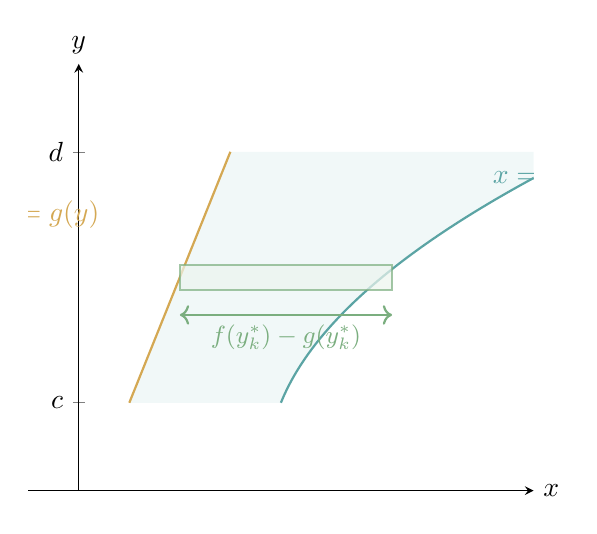
\begin{tikzpicture}
  \begin{axis}[
    width=8cm, height=7cm,
    axis lines=middle,
    xlabel={$x$}, ylabel={$y$},
    ytick={1,3}, yticklabels={$c$,$d$},
    xtick=\empty,
    xmin=-0.5, xmax=4.5, ymin=0.3, ymax=3.7,
    every axis x label/.style={at={(ticklabel* cs:1)}, anchor=west},
    every axis y label/.style={at={(ticklabel* cs:1)}, anchor=south},
  ]
    % Right curve: x = f(y)
    \addplot[name path=R, AtlasTeal, thick, samples=100, domain=1:3, 
      variable=\y] ({0.5*\y*\y - 0.5*\y + 2}, {\y});
    % Left curve: x = g(y)
    \addplot[name path=L, AtlasWarm, thick, samples=100, domain=1:3,
      variable=\y] ({0.5*\y}, {\y});
    \addplot[AtlasTealLight, opacity=0.6] fill between[of=R and L];
    
    \node[right, AtlasTeal] at (axis cs:4,2.8) {$x=f(y)$};
    \node[left, AtlasWarm] at (axis cs:0.3,2.5) {$x=g(y)$};
    
    % Sample horizontal strip
    \draw[AtlasSage, thick, fill=AtlasSageLight, opacity=0.7] 
      (axis cs:1,1.9) rectangle (axis cs:3.1,2.1);
    \draw[<->, thick, AtlasSage] (axis cs:1,1.7) -- 
      node[below, font=\small] {$f(y_k^*) - g(y_k^*)$} (axis cs:3.1,1.7);
  \end{axis}
\end{tikzpicture}
\end{document}
